\section{Theory}
\label{sec:theory}

\begin{figure}[h!]
\centering
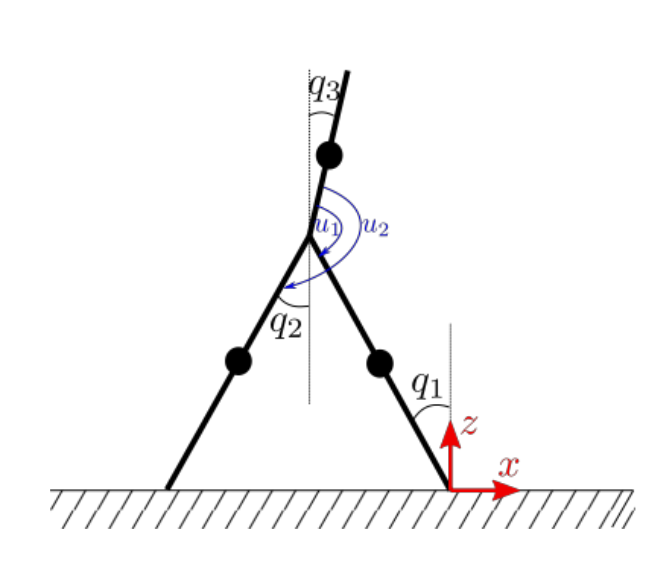
\includegraphics[width = 0.4\columnwidth]{simplified_model}
\label{fig:simplified_model}
\end{figure}

The simplified model of the humanoid is shown in Fig.~\ref{fig:simplified_model}. It is represented by three-links model, two refer to the legs and one for the torso. Each link has a point mass at its center. At each instant, one leg acts as the stance leg that stays stationary, and the other as the swing leg. 

\subsection{Kinematics}
\label{sec:kine}
The kinematics can be easily calculated by considering the stance foot location as the origin of the coordinate frame, as shown in Fig.~\ref{fig:simplified_model}. The points of interests are then the location of each mass ($\bm{p}_1, \bm{p}_2, \bm{p}_3$), the hip ($\bm{p}_h$), and the swing foot ($\bm{p}_{swf}$). Each point $\bm{p}$ consists of the $x$ and $z$ coordinates for this 2D model. By simple geometry, we obtain
\begin{align}
x_1 = &  0.5*l_1*sin(q_1) \\
z_1 = & 0.5*l_1*cos(q_1) \\
x_2 = & l_1*sin(q_1)-0.5*l_2*sin(q_2) \\
z_2 = & l_1*cos(q_1)-0.5*l_2*cos(q_2) \\
x_3 = & l_1*sin(q_1)+ 0.5*l_3*sin(q_3) \\
z_3 = & l_1*cos(q_1)+ 0.5*l_3*cos(q_3) \\
x_h = & l_1*sin(q_1) \\
z_h = & l_1*cos(q_1) \\
x_{swf} = & l_1*sin(q_1)-l_2*sin(q_2) \\
z_{swf} = & l_1*cos(q_1)-l_2*cos(q_2) \\
x_t = & l_1*sin(q_1)+ l_3*sin(q_3) \\
z_t = & l_1*cos(q_1)+ l_3*cos(q_3).
\end{align}

The corresponding velocities can then be computed using chain rule, i.e.
\begin{equation}
\dv{\bm{p}}{t} = \pdv{\bm{p}}{\bm{q}} \pdv{\bm{q}}{t}.
\end{equation}

Using the symbolic programming in matlab or python, it can be done automatically. 

\subsection{Dynamics}
\label{sec:dyn}
To obtain the dynamic equation of the locomotion model, the dynamics is divided into two phases: the swing phase and the impact phase. In the swing phase, we assume that the stance foot is not moving (there is sufficient contact force to keep it stationary), while the swing foot is moving to the next contact location. At the point of impact, we assume an instantaneous impact that preserves the momentum, as described in the next section. 

To describe the dynamics of the swing phase, we can rely on Lagrangian dynamics. First, we found the expression of the total kinetic and potential energy ($T$ and $V$),
\begin{align}
T = & \sum_{i=1}^{3} \frac{1}{2} m_i \dv{\bm{p}_i}{t}^2 \\
V = & \sum_{i=1}^{3} m_i g z_i.
\end{align}

The Lagrangian is then calculated as 
\begin{equation}
L = T - V . 
\end{equation}

With this, the Lagrangian equation of motion can be calculated as
\begin{equation}
\frac{d}{dt} (\pdv{L}{\dot{q}_i}) - \pdv{L}{q_i} = \tau_i,
\label{eq:total_lagrange}
\end{equation}
where $\tau_i$ is the generalized torque. The equations can be computed using the symbolic programming. 

After obtaining the equations for $i = 1, 2, 3$, we can rearrange them in the following form, 
\begin{equation}
\bm{M}(\bm{q})\ddot{\bm{q}} + \bm{C}({\bm{q}},\dot{\bm{q}})\dot{\bm{q}} + \bm{G}({\bm{q}}) = \bm{\tau}. 
\label{eq:total_standard}
\end{equation}

The terms $\bm{M}(\bm{q}), \bm{C}(\dot{\bm{q}},\ddot{\bm{q}})$, and $\bm{G}({\bm{q}})$ cna be computed from \eqref{eq:total_standard} as follows. $\bm{G}(\bm{q})$ is computed by setting $(\dot{\bm{q}}, \dot{\bm{q}}, \bm{\tau})$ in \eqref{eq:total_standard} to zero. 
$\bm{M}(\bm{q})$ is computed by setting $(\dot{\bm{q}},\bm{\tau})$ in \eqref{eq:total_standard} to zero, and substract the term $\bm{G}(\bm{q})$ from the equation. Finally, $\bm{C}(\dot{\bm{q}})$ is computed by setting 
$(\ddot{\bm{q}}, \bm{\tau})$ to zero, substract the term $\bm{G}(\bm{q})$ from the equation, and divide by the corresponding $\dot{\bm{q}}$. 

\subsection{Impact Map}
\label{sec:impact}

\begin{figure}[h!]
\centering
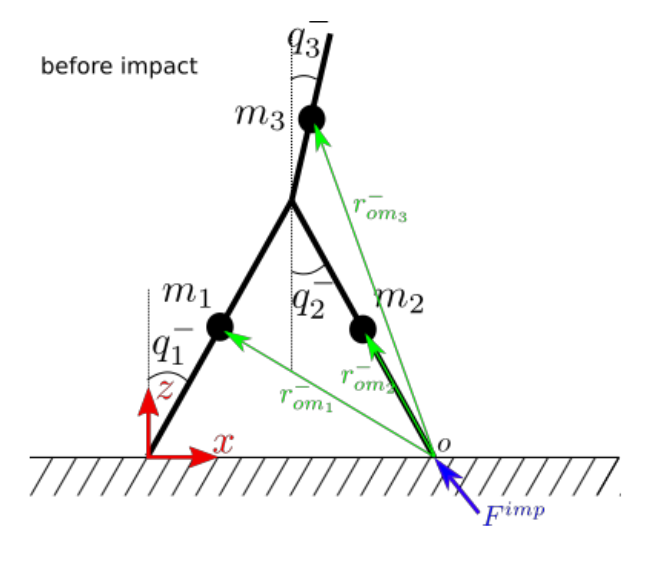
\includegraphics[width = 0.4\columnwidth]{before_impact}
\hspace{0.5cm}
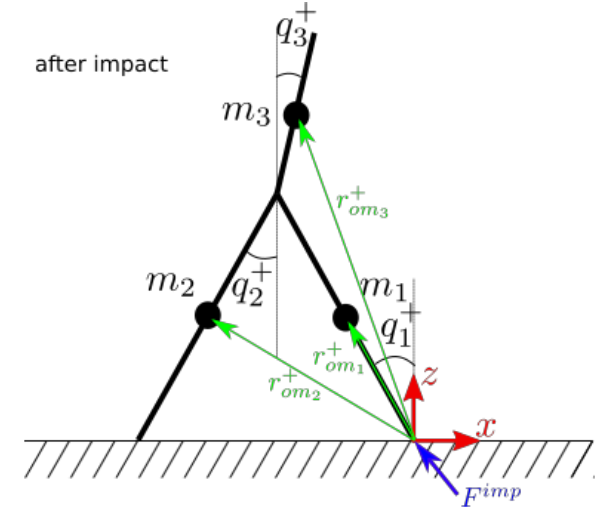
\includegraphics[width = 0.4\columnwidth]{after_impact}
\label{fig:impact}
\end{figure}


\begin{figure}[h!]
\centering
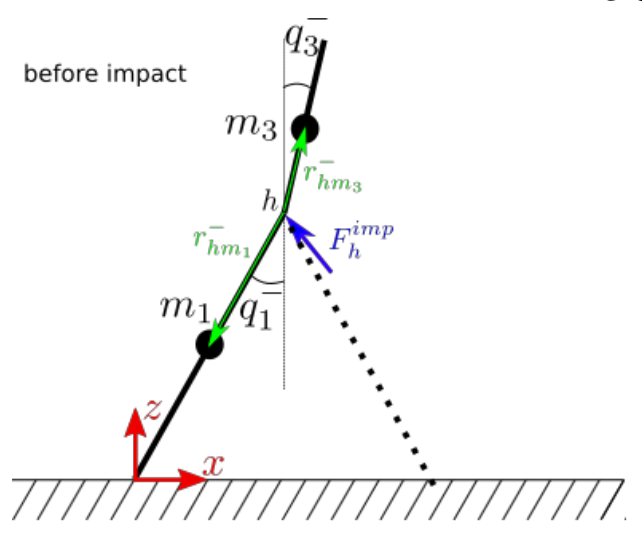
\includegraphics[width = 0.4\columnwidth]{before_impact2}
\hspace{0.5cm}
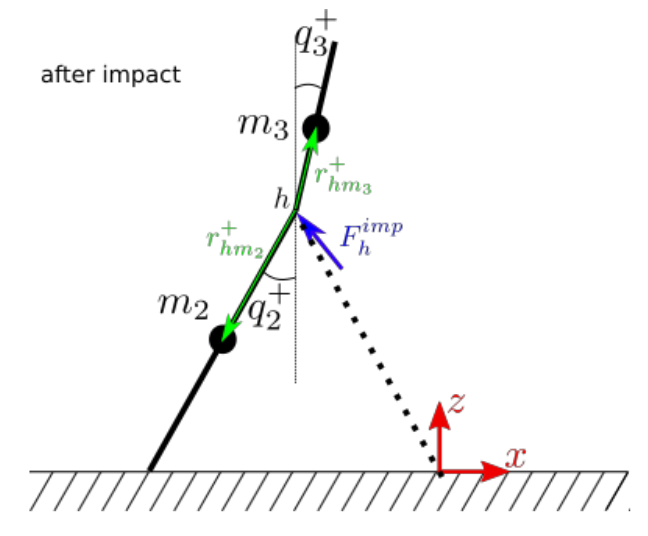
\includegraphics[width = 0.4\columnwidth]{after_impact2}
\label{fig:impact2}
\end{figure}


In our model, after the impact we switch the swing foot to become the stance foot, as shown in Fig.~\ref{fig:impact} (left: before impact, right: after impact). The angles are therefore changed as follows,
\begin{align}
q_1^+ = & q_2^- \\
q_2^+ = & q_1^- \\
q_3^+ = & q_3^-.
\end{align}

The impact map for the angular velocity can be computed by considering the conservation of angular momentum at the impact at two locations: the impact point (the location of the swing foot at the impact), and at the hip. 

Looking at Fig.~\ref{fig:impact} (left), the momentum before the impact can be written as:
\begin{align}
H_a^- = \sum_{i=1}^{3} m_i \bm{r}_{{om}_i}^{-} \cross \dot{\bm{r}_i}^{-} \\
H_b^- = m_1 \bm{r}_{hm_1}^- \cross \dot{\bm{r}_1^-} \\
H_c^- = m_3 \bm{r}_{hm_3}^- \cross \dot{\bm{r}_3^-},
\end{align}
and after impact as
\begin{align}
H_a^+ = \sum_{i=1}^{3} m_i \bm{r}_{{om}_i}^{+} \cross \dot{\bm{r}_i}^{+} \\ 
H_b^+ = m_1 \bm{r}_{hm_2}^+ \cross \dot{\bm{r}_2^+} \\
H_c^+ = m_3 \bm{r}_{hm_3}^+ \cross \dot{\bm{r}_3^+}.
\end{align}

We can rearrange the equations to obtain $\bm{H}^- = \bm{A}_{\_} \dot{\bm{q}}^-$ and $\bm{H}^- = \bm{A}_{+} \dot{\bm{q}}^+$. Then we can obtain the velocities after the impact by solving the linear equation $\bm{H}^- = \bm{H}^+$, 
\begin{equation}
\dot{\bm{q}}^+ = \bm{A}_{+}^{-1} \bm{A}_{\_}  \dot{\bm{q}}^-. 
\end{equation}

\subsubsection{Exercise Answers}
\begin{itemize}
\item Q: \emph{What can you say about the potential energy before and after impact?} 
The potential energy before and after impact does not differ, because the position of each mass remains the same. What changes after the impact is only the kinetic energy.
\item Q: \emph{Try $q_m = [pi/6, -pi/6, pi/10], dq_m = [1, 0.2, 0]$. What percentage of the kinetic energy of the biped is lost due to the impact?}  
There is 27.92\% of the kinetic energy lost due to the impact. 
\item Q: \emph{Plot the percentage of the kinetic energy loss due to impact as a function of angle $\alpha$ where $q^- = [\alpha, -\alpha, 0]$  and $\alpha$ varies from 0 to $\pi/4$. Assume that $\dot q^- = [1, 0.2, 0]$. Include your plot.}
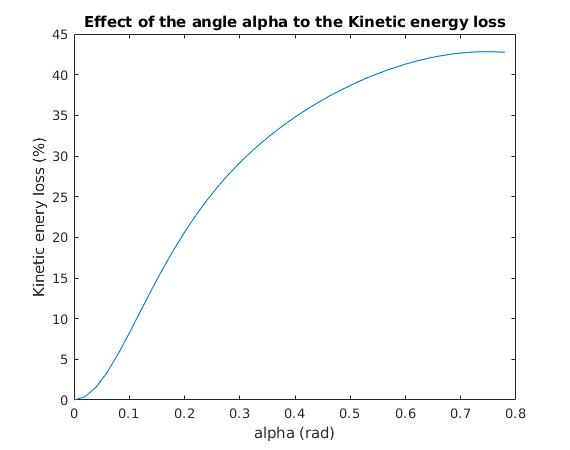
\includegraphics[width=0.6\columnwidth]{alpha_kineticloss}
\item Q: \emph{The bigger $\alpha$ is the bigger is the step length. Based on your answer to question 3, what is the relation between step length and energy loss at impact given a fixed $\dot q^-$?}
As the step length grows bigger, the energy loss increases.    
\end{itemize}

\subsection{Model Validation and Animation}
\label{sec:validation}


\subsubsection{Exercise Answers}
\begin{itemize}
\item \emph{ In the animations, what does a real-time factor of 1 mean? How about a real-time factor less than 1?}
The real time factor describes the ratio between the actual time taken by the motion and the animation time. Real time factor of 1 means that the duration of the animation that appears to us is exactly the same as the duration of the actual step according to the model. Real time factor less than 1 means that the animation appears slower than the actual motion.
\item \emph{How does “skip” in animate.m effect the real-time factor and the speed of the animation?}
The variable "skip" determines how many data points that we do not show in the animation. The larger this value is, the sparser the animation is, and the faster it is. Hence, as "skip" increases, the real time factor will increase and the animation speed becomes faster.
\item \emph{What is the role of r0 in animate.m?}
r0 is the location of the supporting foot. This is necessary because the coordinates of the other points are described with respect to this point. As the supporting foot changes at the impact, the value of r0 is updated correspondingly. 
\end{itemize}

\subsection{Numerical Integration}
\label{sec:num_int}

\subsection{Control and Optimization}
\label{sec:control_opt}

The system during the swing phase is underactuated, i.e. there are three degrees of freedom to control but only two control inputs, as shown in Fig.~\ref{fig:control}. In the standard controller, we first choose the first control input $u_1$ to control the torso angle to be at a desired value $\alpha$, whereas the second control input $u_2$ is used to control the swing foot angle $q_2$. Expressing these as virtual constraints in terms of new variables $y_1$ and $y_2$, we set
\begin{align}
y_1 = q_3 - \alpha \\
y_2 = -q_2 - q_1. 
\end{align}

Differentiating this constraint, we obtain
\begin{align}
\dot{y}_1 = \dot{q}_3  \\
\dot{y}_2 = -\dot{q}_2 - \dot{q}_1. 
\end{align}

We then set the controller as PD control to drive $y_1, y_2$ to zeros,
\begin{align}
u_1 = k_1^P y_1 + k_1^D \dot{y}_1 \\
u_2 = k_2^P y_2 + k_2^D \dot{y}_2.
\end{align}

Now what is left is to choose the parameters $(k_1^P, k_1^D, k_2^P, k_2^D, \text{and} \alpha)$, as well as the initial state $(\bm{q}^0, \dot{\bm{q}}^0)$. We use the function $\emph{fmin}$ in Matlab to optimize these parameters, given an objective function. 








